\section{Porównanie wyników}

\subsection{Platforma testowa}

Testy przeprowadzono na komputerze stancjonarnym o następującej specyfikacji:

\begin{itemize}
	\item System operacyjny -- Windows 10 Home 64-bit.
	\item Procesor -- Intel Core i5 4590, taktowanie 3.30GHz.
	\item Pamięć RAM -- 8 GB 2-Kanałowy DDR3, taktowanie 1600 MHz.
\end{itemize}

\subsection{Badane wartości}

Jakość kompresji określono za pomocą współczynnika kompresji, którego można przedstawić przy pomocy wzoru:
\[
CR = \frac{ Skompresowany Rozmiar }{ Nieskompresowany Rozmiar } 
\]

W tym przypadku, im niższa wartość tym lepszy algorytm. Współczynnik można również zapisać procentowo.

Drugą mierzoną wartością był czas kompresji obliczany w milisekundach.

\subsection{Obrazy barwne}

Podstawą dla obrazów barwnych był format \textbf{PPM} -- odmiana bitmapy, będącej formą zapisu grafiki rastrowej. PPM jest przeznaczony dla obrazów kolorowych i zawiera maksymalnie do 24 bitów na piksel w trybie binarnym (8 bitów na każdy kolor).

\begin{table}[!h]
	\centering
	\caption{\textbf{Clegg}}
	\label{my-label}
	\begin{tabular}{|c|c|c|c|c|}                                             
		\hline
		& \textbf{Rozmiar przed} & \textbf{Rozmiar po} & \textbf{Wspł. kompresji} & \textbf{Czas {[}ms{]}} \\ \hline 
		\textbf{PNG}      &          \multicolumn{1}{c|}{\multirow{2}{*}{2099 KB}}             &      475 KB               &         22,62 \%                 &              216               \\\cline{3-5}
		\textbf{JPEG-LS}  &                        &        638  KB         &      30,39 \%                  &         58                 \\\cline{3-5}
		\textbf{JPEG2000} &                        &        1370 KB             &       65,25 \%                   &        273              \\ \hline
	\end{tabular}
\end{table}

\begin{table}[!h]
	\centering
	\caption{\textbf{Frymire}}
	\label{my-label}
	\begin{tabular}{|c|c|c|c|c|}                                             
		\hline
		& \textbf{Rozmiar przed} & \textbf{Rozmiar po} & \textbf{Wspł. kompresji} & \textbf{Czas {[}ms{]}} \\ \hline 
		\textbf{PNG}      &          \multicolumn{1}{c|}{\multirow{2}{*}{3620 KB}}             &         380 KB              &        10,49 \%                   &            176                 \\\cline{3-5}
		\textbf{JPEG-LS}  &                        &        914 KB             &         25,25 \%                 &           59               \\\cline{3-5}
		\textbf{JPEG2000} &                        &         1561 KB               &          43,11 \%                &       719               \\ \hline
	\end{tabular}
\end{table}

\begin{table}[!h]
	\centering
	\caption{\textbf{Lena3}}
	\label{my-label}
	\begin{tabular}{|c|c|c|c|c|}                                             
		\hline
		& \textbf{Rozmiar przed} & \textbf{Rozmiar po} & \textbf{Wspł. kompresji} & \textbf{Czas {[}ms{]}} \\ \hline 
		\textbf{PNG}      &          \multicolumn{1}{c|}{\multirow{2}{*}{769 KB}}             &      466 KB               &        60,54 \%                  &         103                    \\\cline{3-5}
		\textbf{JPEG-LS}  &                        &         436 KB            &      56,81 \%                   &         30                 \\\cline{3-5}
		\textbf{JPEG2000} &                        &     435 KB             &         57,93 \%                 &       440               \\ \hline
	\end{tabular}
\end{table}

\begin{table}[!h]
	\centering
	\caption{\textbf{Monarch}}
	\label{my-label}
	\begin{tabular}{|c|c|c|c|c|}                                             
		\hline
		& \textbf{Rozmiar przed} & \textbf{Rozmiar po} & \textbf{Wspł. kompresji} & \textbf{Czas {[}ms{]}} \\ \hline 
		\textbf{PNG}      &          \multicolumn{1}{c|}{\multirow{2}{*}{1153 KB}}             &      605 KB               &          52,44 \%                &            230                 \\\cline{3-5}
		\textbf{JPEG-LS}  &                        &       543 KB             &        46,94 \%                 &        44                  \\\cline{3-5}
		\textbf{JPEG2000} &                        &      432 KB               &        37,44 \%                 &       482               \\ \hline
	\end{tabular}
\end{table}

\begin{table}[!h]
	\centering
	\caption{\textbf{Peppers3}}
	\label{my-label}
	\begin{tabular}{|c|c|c|c|c|}                                             
		\hline
		& \textbf{Rozmiar przed} & \textbf{Rozmiar po} & \textbf{Wspł. kompresji} & \textbf{Czas {[}ms{]}} \\ \hline 
		\textbf{PNG}      &          \multicolumn{1}{c|}{\multirow{2}{*}{769 KB}}             &         418 KB            &        54,33 \%                  &         149                    \\\cline{3-5}
		\textbf{JPEG-LS}  &                        &          377 KB           &         49,01 \%                 &          29                \\\cline{3-5}
		\textbf{JPEG2000} &                        &        328 KB             &      42,64 \%                    &      367                \\ \hline
	\end{tabular}
\end{table}

\begin{table}[!h]
	\centering
	\caption{\textbf{Sail}}
	\label{my-label}
	\begin{tabular}{|c|c|c|c|c|}                                             
		\hline
		& \textbf{Rozmiar przed} & \textbf{Rozmiar po} & \textbf{Wspł. kompresji} & \textbf{Czas {[}ms{]}} \\ \hline 
		\textbf{PNG}      &          \multicolumn{1}{c|}{\multirow{2}{*}{1153 KB}}             &       792 KB              &         68,66 \%                 &           156                  \\\cline{3-5}
		\textbf{JPEG-LS}  &                        &        750  KB           &         64,93 \%                &          45                \\\cline{3-5}
		\textbf{JPEG2000} &                        &        512 KB             &      44,37 \%                   &      542                \\ \hline
	\end{tabular}
\end{table}

\begin{table}[!h]
	\centering
	\caption{\textbf{Serrano}}
	\label{my-label}
	\begin{tabular}{|c|c|c|c|c|}                                             
		\hline
		& \textbf{Rozmiar przed} & \textbf{Rozmiar po} & \textbf{Wspł. kompresji} & \textbf{Czas {[}ms{]}} \\ \hline 
		\textbf{PNG}      &          \multicolumn{1}{c|}{\multirow{2}{*}{1464 KB}}             &       155 KB              &            10,58 \%              &           95                  \\\cline{3-5}
		\textbf{JPEG-LS}  &                        &         287 KB            &      19,60 \%                   &          23                \\\cline{3-5}
		\textbf{JPEG2000} &                        &         624 KB            &         42,61 \%                 &       740               \\ \hline
	\end{tabular}
\end{table}

\begin{table}[!h]
	\centering
	\caption{\textbf{Tulips}}
	\label{my-label}
	\begin{tabular}{|c|c|c|c|c|}                                             
		\hline
		& \textbf{Rozmiar przed} & \textbf{Rozmiar po} & \textbf{Wspł. kompresji} & \textbf{Czas {[}ms{]}} \\ \hline 
		\textbf{PNG}      &          \multicolumn{1}{c|}{\multirow{2}{*}{1153 KB}}             &        667 KB             &      57,88 \%                   &          202                   \\\cline{3-5}
		\textbf{JPEG-LS}  &                        &      603  KB             &       52,35 \%                  &          46                \\\cline{3-5}
		\textbf{JPEG2000} &                        &      478 KB               &       41,46 \%                  &     547                 \\ \hline
	\end{tabular}
\end{table}




\begin{figure}[!h]
	\centering
	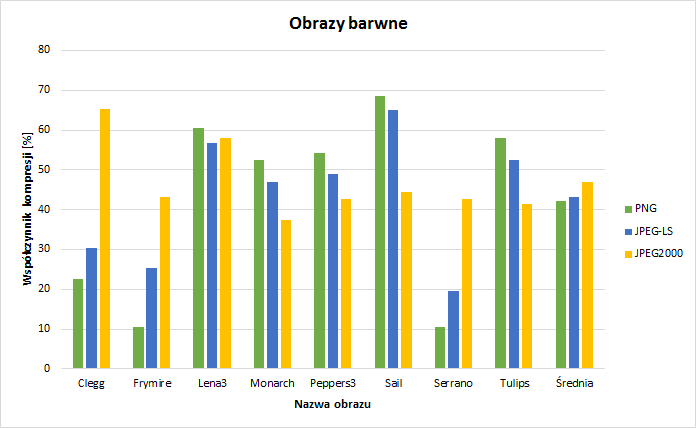
\includegraphics[width=1.1\textwidth]{./color.png}
	\caption{Wykres słupkowy dla obrazów kolorowych}
	\label{img:color}
\end{figure}

\clearpage








\subsection{Obrazy czarno-białe}

Podstawą dla obrazów z zestawu Waterloo Greyset 2 był format \textbf{PGM} -- odmiana bitmapy, będącej formą zapisu grafiki rastrowej. PGM jest przeznaczony dla w obrazów odcieniach szarości i zawiera 8 bitów na piksel.

\begin{table}[!h]
	\centering
	\caption{\textbf{Barb}}
	\label{my-label}
	\begin{tabular}{|c|c|c|c|c|}                                             
		\hline
		& \textbf{Rozmiar przed} & \textbf{Rozmiar po} & \textbf{Wspł. kompresji} & \textbf{Czas {[}ms{]}} \\ \hline 
		\textbf{PNG}      &          \multicolumn{1}{c|}{\multirow{2}{*}{257 KB}}             &      170 KB               &    66,28 \%                     &           58                  \\\cline{3-5}
		\textbf{JPEG-LS}  &                        &       152 KB              &        59,17 \%                 &        10                  \\\cline{3-5}
		\textbf{JPEG2000} &                        &     150 KB                &        58,24 \%                 &        155              \\ \hline
	\end{tabular}
\end{table}

\begin{table}[!h]
	\centering
	\caption{\textbf{Boat}}
	\label{my-label}
	\begin{tabular}{|c|c|c|c|c|}                                             
		\hline
		& \textbf{Rozmiar przed} & \textbf{Rozmiar po} & \textbf{Wspł. kompresji} & \textbf{Czas {[}ms{]}} \\ \hline 
		\textbf{PNG}      &          \multicolumn{1}{c|}{\multirow{2}{*}{257 KB}}             &       149 KB              &      57,94 \%                    &           67                  \\\cline{3-5}
		\textbf{JPEG-LS}  &                        &       136 KB              &         53,19 \%                &         10                 \\\cline{3-5}
		\textbf{JPEG2000} &                        &      141 KB               &        55,07 \%                &        151              \\ \hline
	\end{tabular}
\end{table}

\begin{table}[!h]
	\centering
	\caption{\textbf{France}}
	\label{my-label}
	\begin{tabular}{|c|c|c|c|c|}                                             
		\hline
		& \textbf{Rozmiar przed} & \textbf{Rozmiar po} & \textbf{Wspł. kompresji} & \textbf{Czas {[}ms{]}} \\ \hline 
		\textbf{PNG}      &          \multicolumn{1}{c|}{\multirow{2}{*}{326 KB}}             &     18  KB              &    5,27 \%                     &            40                 \\\cline{3-5}
		\textbf{JPEG-LS}  &                        &        58 KB             &       17,63 \%                  &          5                \\\cline{3-5}
		\textbf{JPEG2000} &                        &     83 KB                &      25,25 \%                   &         142             \\ \hline
	\end{tabular}
\end{table}

\begin{table}[!h]
	\centering
	\caption{\textbf{Frog}}
	\label{my-label}
	\begin{tabular}{|c|c|c|c|c|}                                             
		\hline
		& \textbf{Rozmiar przed} & \textbf{Rozmiar po} & \textbf{Wspł. kompresji} & \textbf{Czas {[}ms{]}} \\ \hline 
		\textbf{PNG}      &          \multicolumn{1}{c|}{\multirow{2}{*}{303 KB}}             &        227 KB             &    75,01 \%                     &           57                  \\\cline{3-5}
		\textbf{JPEG-LS}  &                        &      229 KB               &       75,75 \%                  &         12                 \\\cline{3-5}
		\textbf{JPEG2000} &                        &      237 KB               &       78,22 \%                  &      125                \\ \hline
	\end{tabular}
\end{table}

\begin{table}[!h]
	\centering
	\caption{\textbf{Goldhill2}}
	\label{my-label}
	\begin{tabular}{|c|c|c|c|c|}                                             
		\hline
		& \textbf{Rozmiar przed} & \textbf{Rozmiar po} & \textbf{Wspł. kompresji} & \textbf{Czas {[}ms{]}} \\ \hline 
		\textbf{PNG}      &          \multicolumn{1}{c|}{\multirow{2}{*}{257 KB}}             &        157 KB             &      61,08 \%                   &               54              \\\cline{3-5}
		\textbf{JPEG-LS}  &                        &       151 KB              &         58,82 \%                &            10              \\\cline{3-5}
		\textbf{JPEG2000} &                        &       155 KB              &         60,47 \%                &       171               \\ \hline
	\end{tabular}
\end{table}

\begin{table}[!h]
	\centering
	\caption{\textbf{Lena2}}
	\label{my-label}
	\begin{tabular}{|c|c|c|c|c|}                                             
		\hline
		& \textbf{Rozmiar przed} & \textbf{Rozmiar po} & \textbf{Wspł. kompresji} & \textbf{Czas {[}ms{]}} \\ \hline 
		\textbf{PNG}      &          \multicolumn{1}{c|}{\multirow{2}{*}{257 KB}}             &      148 KB               &       57,57 \%                  &           63                   \\\cline{3-5}
		\textbf{JPEG-LS}  &                        &        136 KB             &         52,95 \%                &       10                   \\\cline{3-5}
		\textbf{JPEG2000} &                        &      139 KB               &          53,95 \%               &       150               \\ \hline
	\end{tabular}
\end{table}

\begin{table}[!h]
	\centering
	\caption{\textbf{Library}}
	\label{my-label}
	\begin{tabular}{|c|c|c|c|c|}                                             
		\hline
		& \textbf{Rozmiar przed} & \textbf{Rozmiar po} & \textbf{Wspł. kompresji} & \textbf{Czas {[}ms{]}} \\ \hline 
		\textbf{PNG}      &          \multicolumn{1}{c|}{\multirow{2}{*}{160 KB}}             &      103 KB               &    64,18 \%                     &           37                  \\\cline{3-5}
		\textbf{JPEG-LS}  &                        &     102 KB                &        63,69 \%                 &           6               \\\cline{3-5}
		\textbf{JPEG2000} &                        &     114 KB                &        71,20 \%                 &        127              \\ \hline
	\end{tabular}
\end{table}

\begin{table}[!h]
	\centering
	\caption{\textbf{Mandrill}}
	\label{my-label}
	\begin{tabular}{|c|c|c|c|c|}                                             
		\hline
		& \textbf{Rozmiar przed} & \textbf{Rozmiar po} & \textbf{Wspł. kompresji} & \textbf{Czas {[}ms{]}} \\ \hline 
		\textbf{PNG}      &          \multicolumn{1}{c|}{\multirow{2}{*}{257 KB}}             &     200 KB                &        76,28 \%                 &         49                    \\\cline{3-5}
		\textbf{JPEG-LS}  &                        &       194 KB             &        75,18 \%                &           10               \\\cline{3-5}
		\textbf{JPEG2000} &                        &       196 KB              &          76,37 \%               &     182                 \\ \hline
	\end{tabular}
\end{table}

\begin{table}[!h]
	\centering
	\caption{\textbf{Mountain}}
	\label{my-label}
	\begin{tabular}{|c|c|c|c|c|}                                             
		\hline
		& \textbf{Rozmiar przed} & \textbf{Rozmiar po} & \textbf{Wspł. kompresji} & \textbf{Czas {[}ms{]}} \\ \hline 
		\textbf{PNG}      &          \multicolumn{1}{c|}{\multirow{2}{*}{301 KB}}             &       248 KB              &      82,53 \%                   &            65                 \\\cline{3-5}
		\textbf{JPEG-LS}  &                        &       240 KB              &          80,64 \%               &            12              \\\cline{3-5}
		\textbf{JPEG2000} &                        &       252 KB              &          83,76 \%               &       241               \\ \hline
	\end{tabular}
\end{table}

\begin{table}[!h]
	\centering
	\caption{\textbf{Peppers2}}
	\label{my-label}
	\begin{tabular}{|c|c|c|c|c|}                                             
		\hline
		& \textbf{Rozmiar przed} & \textbf{Rozmiar po} & \textbf{Wspł. kompresji} & \textbf{Czas {[}ms{]}} \\ \hline 
		\textbf{PNG}      &          \multicolumn{1}{c|}{\multirow{2}{*}{257 KB}}             &      156 KB               &     60,56 \%                    &          56                   \\\cline{3-5}
		\textbf{JPEG-LS}  &                        &       144 KB              &       56,17 \%                  &             11             \\\cline{3-5}
		\textbf{JPEG2000} &                        &       148 KB              &       57,73 \%                  &        150              \\ \hline
	\end{tabular}
\end{table}

\begin{table}[!h]
	\centering
	\caption{\textbf{Washsat}}
	\label{my-label}
	\begin{tabular}{|c|c|c|c|c|}                                             
		\hline
		& \textbf{Rozmiar przed} & \textbf{Rozmiar po} & \textbf{Wspł. kompresji} & \textbf{Czas {[}ms{]}} \\ \hline 
		\textbf{PNG}      &          \multicolumn{1}{c|}{\multirow{2}{*}{257 KB}}             &         104 KB            &     40,35 \%                    &          88                   \\\cline{3-5}
		\textbf{JPEG-LS}  &                        &      133 KB               &          51,54 \%               &           9               \\\cline{3-5}
		\textbf{JPEG2000} &                        &      142 KB               &          55,39 \%               &     169                 \\ \hline
	\end{tabular}
\end{table}

\begin{table}[!h]
	\centering
	\caption{\textbf{Zelda}}
	\label{my-label}
	\begin{tabular}{|c|c|c|c|c|}                                             
		\hline
		& \textbf{Rozmiar przed} & \textbf{Rozmiar po} & \textbf{Wspł. kompresji} & \textbf{Czas {[}ms{]}} \\ \hline 
		\textbf{PNG}      &          \multicolumn{1}{c|}{\multirow{2}{*}{257 KB}}             &      137 KB               &     53,17 \%                    &          63                   \\\cline{3-5}
		\textbf{JPEG-LS}  &                        &      129 KB               &       50,17 \%                  &         9                 \\\cline{3-5}
		\textbf{JPEG2000} &                        &      128 KB               &       49,90 \%                  &        147              \\ \hline
	\end{tabular}
\end{table}


\begin{figure}[!h]
	\centering
	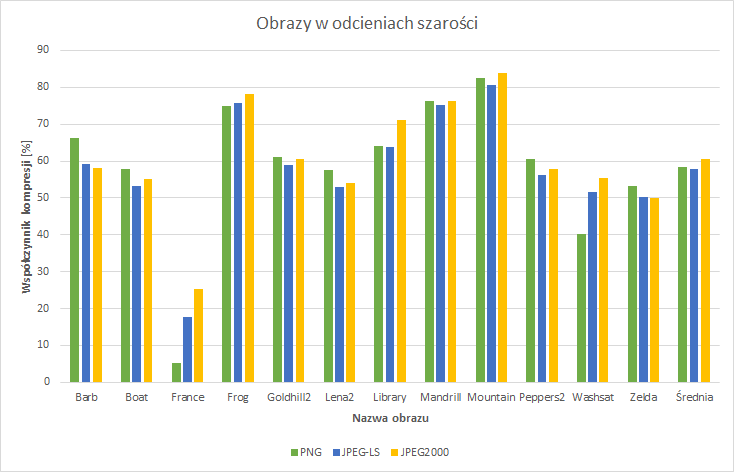
\includegraphics[width=1.1\textwidth]{./greyset.png}
	\caption{Wykres słupkowy dla obrazów w odcieniach szarości}
	\label{img:greyset}
\end{figure}

\clearpage